\chapter{Метод анализа генетических данных для оценки региональных различий адаптации к климатическим условиям}\label{ch:ch3}

\section{Входные данные}\label{sec:ch3/sec1}

Для анализа генетических данных используется информация об однонуклеотидных полиморфизмах (SNP), распределённых по всему геному человеческого организма. Наиболее обширной базой данных генетических вариантов является проект <<1000 геномов>> \autocite{1000genomes2015, Sudmant2015}, целью которого было найти большинство генетических вариантов с частотой не менее $1~\%$ в изучаемых популяциях и создать Международный ресурс геномных образцов (International Genome Sample Resource --- IGSR). В рамках данного проекта были использованы достижения в области технологии секвенирования, что резко снизило его стоимость. Это был первый проект по секвенированию геномов большого числа людей, чтобы собрать большую базу данных генетических вариаций человека. Секвенирование оставалось слишком дорогим для проведения глубокого анализа многих образцов, изучаемых в рамках проекта. Однако, любая конкретная область генома обычно содержит ограниченное количество гаплотипов. Данные были объединены по образцам, чтобы обеспечить эффективное обнаружение большинства вариантов в изучаемом географическом регионе. В рамках проекта каждый образец секвенировался до 4-кратного покрытия генома; на этой глубине секвенирование не может обнаружить все варианты в каждом образце, но может позволить выявить большинство вариантов с частотами всего $1~\%$. На заключительном этапе проекта были объединены данные из 2504 образцов, чтобы обеспечить высокоточное определение генотипов в каждом образце на всех вариативных участках. Образцы для проекта <<1000 геномов>> анонимны и не имеют связанных медицинских или фенотипических данных. Проект придерживается самооценки этнической принадлежности и пола. Во время сбора образцов все участники заявили, что они здоровы. Текущие образцы проекта <<1000 геномов>> не отражают все популяции (список доступных популяций указан в Таблице~\ref{tab:populations}), однако, его целью является обеспечение максимально возможного разнообразия населения. 

\begin{table} [htbp]
	\centering
	\begin{threeparttable}
		\caption{Популяции, представленные в проекте <<1000 геномов>>}%
		\label{tab:populations}%
		\begin{SingleSpace}
			\begin{tabular}{| c | c | c |}
				\hline
				Код 	& Описание 							& Суперпопуляция \\ \hline
				CHB 	& Хань в Пекине, Китай 				& Восточная Азия \\ \hline
				JPT 	& Японцы в Токио, Япония 			& Восточная Азия \\ \hline
				CHS 	& Хань на юге Китая 				& Восточная Азия \\ \hline
				CDX 	& Дай в Сишуанбаньна, Китай 		& Восточная Азия \\ \hline
				KHV 	& Кин в Хошимине, Вьетнам			& Восточная Азия \\ \hline
				CEU 	& \thead{Жители Юты северного и западноевропейского \\ происхождения} 		& Европа \\ \hline
				TSI 	& Тосканцы в Италии	 				& Европа \\ \hline
				FIN 	& Финны в Финляндии 				& Европа \\ \hline
				GBR 	& Британцы в Англии и Шотландии		& Европа \\ \hline
				IBS 	& Иберийское население в Испании	& Европа \\ \hline
				YRI 	& Йоруба в Ибадане, Нигерия			& Африка \\ \hline
				LWK 	& Лухья в Вебуе, Кения		 		& Африка \\ \hline
				GWD 	& Гамбийцы в западных районах Гамбии										& Африка \\ \hline
				MSL 	& Менде в Сьерра-Леоне				& Африка \\ \hline
				ESN 	& Ишан в Нигерии	 				& Африка \\ \hline
				ASW 	& \thead{Американцы африканского происхождения \\ на юго-западе США}		& Африка \\ \hline
				ACB 	& Вест-индские негры на Барбадосе 	& Африка \\ \hline
				MXL 	& \thead{Мексиканское население Лос-Анджелеса, \\ США} 						& Америка (смешанные) \\ \hline
				PUR 	& Пуэрториканцы в Пуэрто-Рико		& Америка (смешанные) \\ \hline
				CLM 	& Колумбийцы в Медельине, Колумбия 	& Америка (смешанные) \\ \hline
				PEL 	& Перуанцы в Лиме, Перу				& Америка (смешанные) \\ \hline
				GIH 	& Гуджаратцы в Хьюстоне, штат Техас & Южная Азия \\ \hline
				PJL 	& Панджабцы в Лахоре, Пакистан		& Южная Азия \\ \hline
				BEB 	& Бенгальцы в Бангладеше 			& Южная Азия \\ \hline
				STU 	& Ланкийские тамилы	в Великобритании										& Южная Азия \\ \hline
				ITU 	& Индийские телугу в Великобритании	& Южная Азия \\ \hline
			\end{tabular}%
		\end{SingleSpace}
	\end{threeparttable}
\end{table}

Отбор проб для проекта <<1000 геномов>> осуществляется в соответствии со следующими критериями:
\begin{itemize}
	\item Все образцы крови взяты у взрослых субъектов.
	\item Для получения 100 неродственных клеточных линий популяции, первичный материал был собран как минимум от 130 неродственных субъектов.
	\item Получены линии <<бессмертных>> клеток, которые можно использовать для получения практически неограниченных количеств ДНК.
	\item Образцы генотипированы с использованием массива генотипов высокой плотности с более чем 500000 маркеров.
\end{itemize}

Информация об однонуклеотидных полиморфизмах сохраняется в формате VCF (Variant Call Format) --- это формат текстового файла, используемого в биоинформатике для хранения генетических вариаций последовательностей генов. Формат был разработан с появлением крупных проектов секвенирования и фенотипирования ДНК, таких как проект <<1000 геномов>>. Файл формата VCF обязательно включает заголовок, который содержит метаданные, описывающие тело файла. Строки заголовков начинаются с символа $\#$, специальные ключевые слова в заголовке обозначаются $\#\#$. Тело файла представляется собой табулированную таблицу, содержащую 8 обязательных столбцов и неограниченное количество дополнительных столбцов. Когда используются дополнительные столбцы, первый дополнительный столбец используется для описания формата данных в следующих столбцах. Обязательные столбцы:
\begin{enumerate}
	\item CHROM --- имя хромосомы, в которой располагается полиморфизм. 
	\item POS --- номер позиции, в которой находится полиморфизм, отсчитываемый от 1.
	\item ID --- идентификатор полиморфизма, например идентификатор rs или, если он неизвестен, ".".
	\item REF --- референсная аллель в данной позиции.
	\item ALT --- список альтернативных аллелей в данной позиции.
	\item QUAL --- оценка качества, связанная с данными аллелями.
	\item FILTER --- флаг, указывающий, какой из заданного набора фильтров был применён.
	\item INFO --- список пар (полей) ключ-значение, описывающих полиморфизм. 
	\item FORMAT --- (необязательный) расширяемый список полей для описания образцов.
	\item SAMPLES --- значения полей, перечисленных в FORMAT, для каждого (необязательного) образца, описанного в файле.
\end{enumerate}

Для проверки результатов работы предлагаемых алгоритмов использовалась часть данных генетических вариаций проекта <<1000 геномов>>, соответствующих репрезентативным популяциям европейского происхождения из разных широт (Рисунок~\ref{fig:europe_map}) --- GBR (Британцы в Англии и Шотландии), FIN (Финны в Финляндии), TSI (Тосканцы в Италии).

\begin{figure}[ht]
	\centerfloat{
		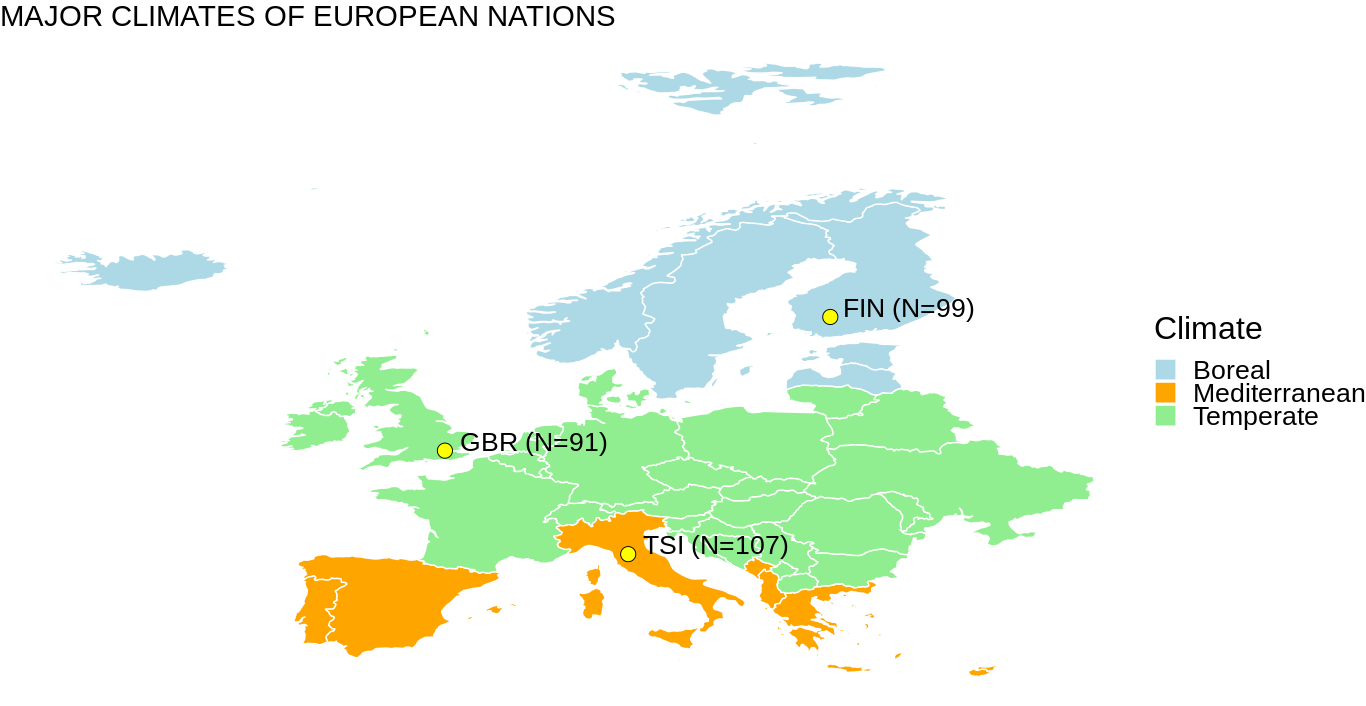
\includegraphics[scale=0.3]{europe_map.png}
	}
	\caption{Карта Европы с рассматриваемыми популяциями и различными климатическими регионами: субарктический (синий), средиземноморский (оранжевый) и умеренный (зелёный).}\label{fig:europe_map}
\end{figure}

\section{Подход к уменьшению размерности входных данных}\label{sec:ch3/sec2}
